{
\begin{figure*}[th]
\begin{center}
\centerline{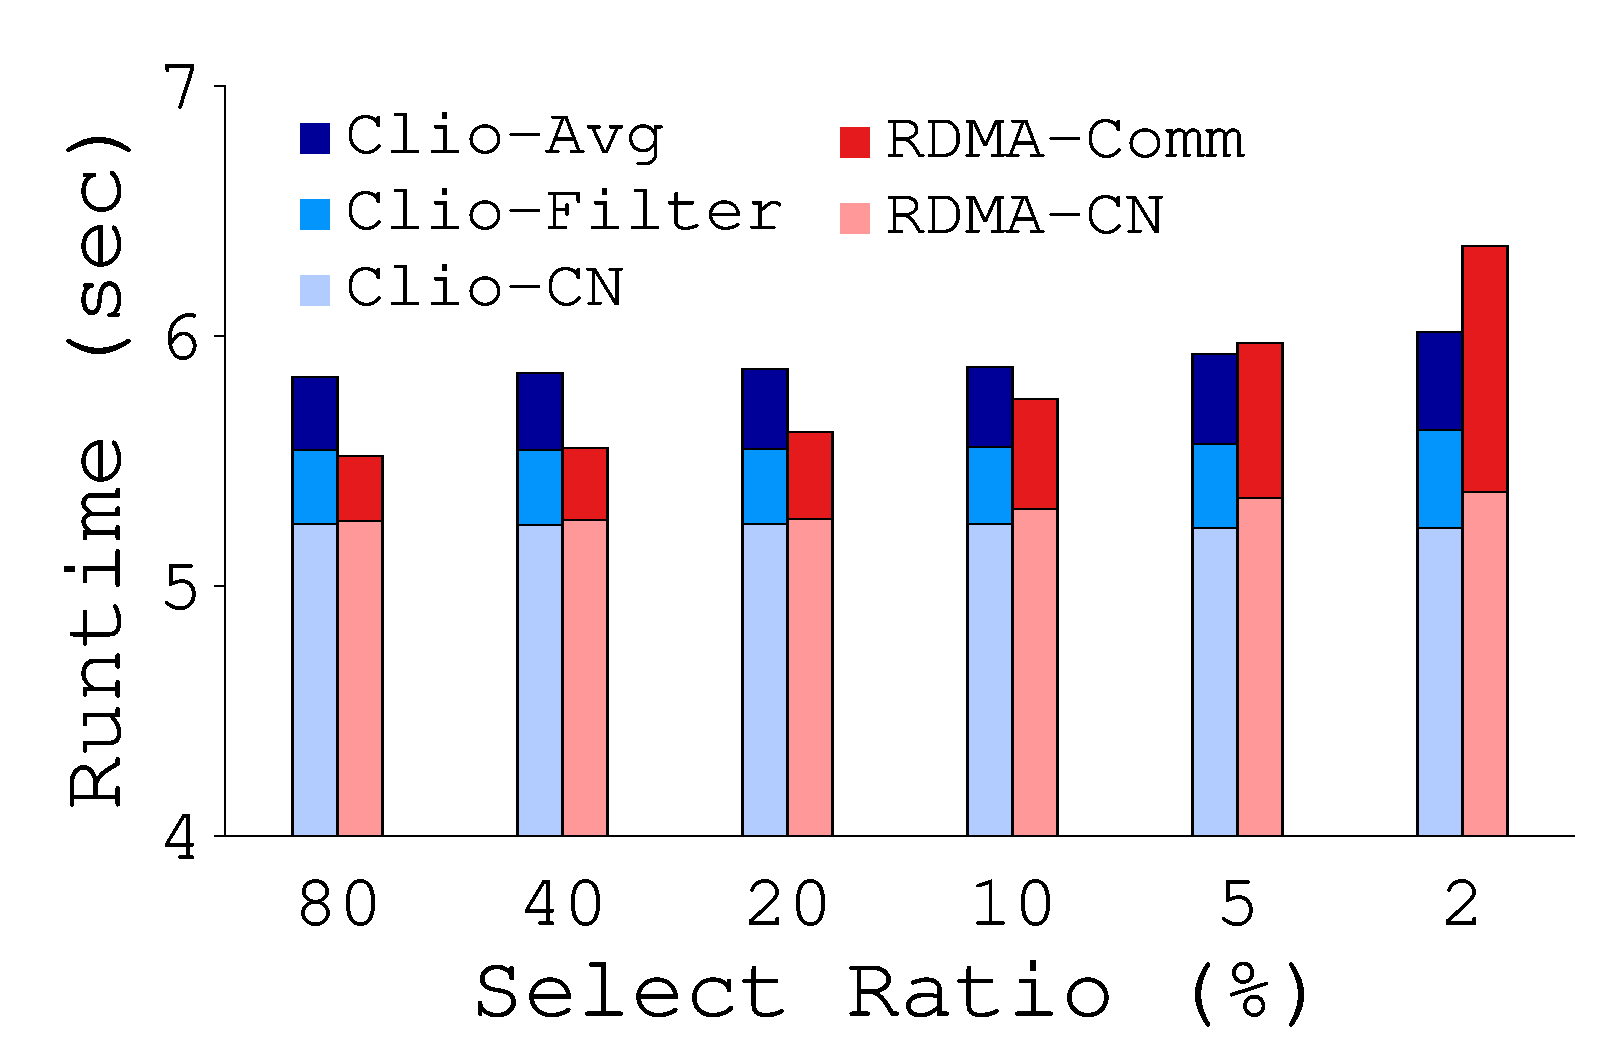
\includegraphics[width=0.5\textwidth]{clio/Figures/g_plot_dp.pdf}}
\mycaption{fig-dataframe}{Select-Aggregate-Shuffle.}
{
Y axis starts at 4 sec. 
CN represents computation done at \CN.
%, as histogram  time is the same.
}
\end{center}
\end{figure*}
}
{
\begin{figure*}[h]
\begin{center}
\centerline{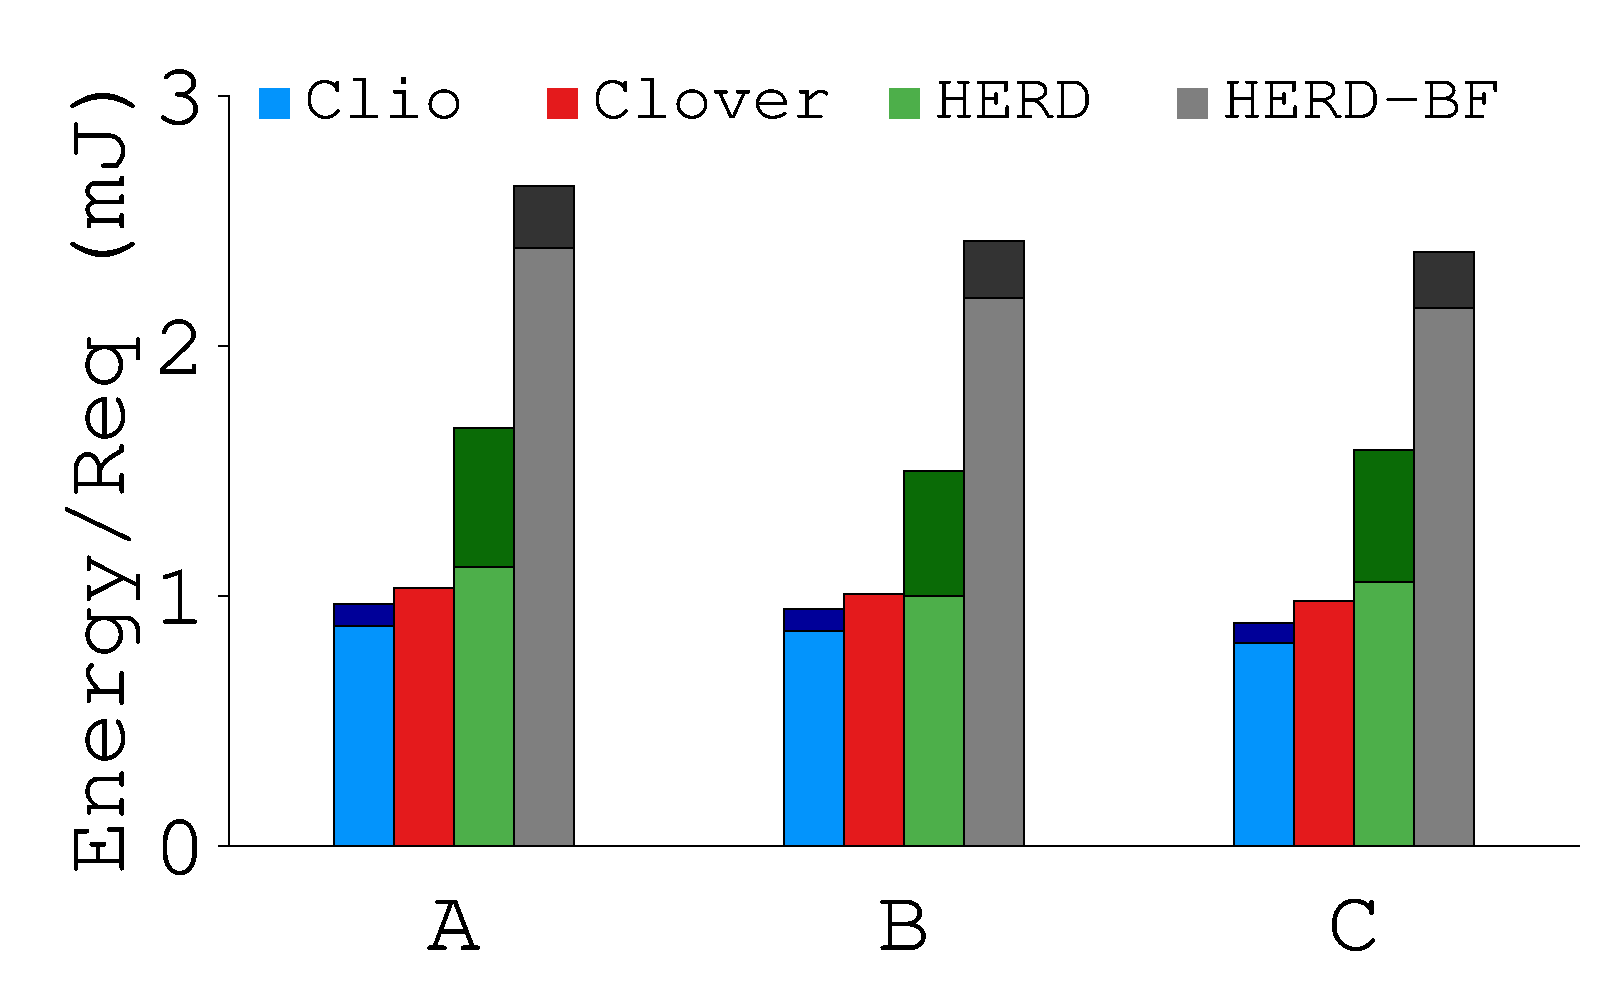
\includegraphics[width=0.5\textwidth]{clio/Figures/g_plot_ycsb_energy.pdf}}
\mycaption{fig-energy}{Energy Comparison.}
{
Darker/lighter shades represent energy spent at \MN{}s and \CN{}s.
}
\end{center}
\end{figure*}
}
{
\begin{table}\small
\begin{center}
\begin{center}
\begin{tabular}{ p{1.2in} | p{0.5in} |p{0.6in} }
 & \textbf{Logic} & \textbf{Memory} \\
\textbf{System/Module} & \textbf{(LUT)} & \textbf{(BRAM)} \\
\hline
\hline
StRoM-RoCEv2 & 39\% & 76\% \\
Tonic-SACK & 48\% & 40\% \\
\hline
\sys\ (Total) & 31\% & 31\% \\
VirtMem & 5.5\% & 3\% \\
NetStack & 2.3\% & 1.7\% \\
\hline
Go-Back-N & 5.8\% & 2.6\% \\
\end{tabular}
\end{center}
\mycaption{fig-fpga-resource}{Clio FPGA Utilization.}
{
}
\end{center}
\end{table}
}